\subsection{SEStar  Class Reference}
\label{class_sestar}\index{SEStar@{SEStar}}
SExtractor star. 


{\tt \#include $<$sestar.h$>$}

Inheritance diagram for SEStar::\begin{figure}[H]
\begin{center}
\leavevmode
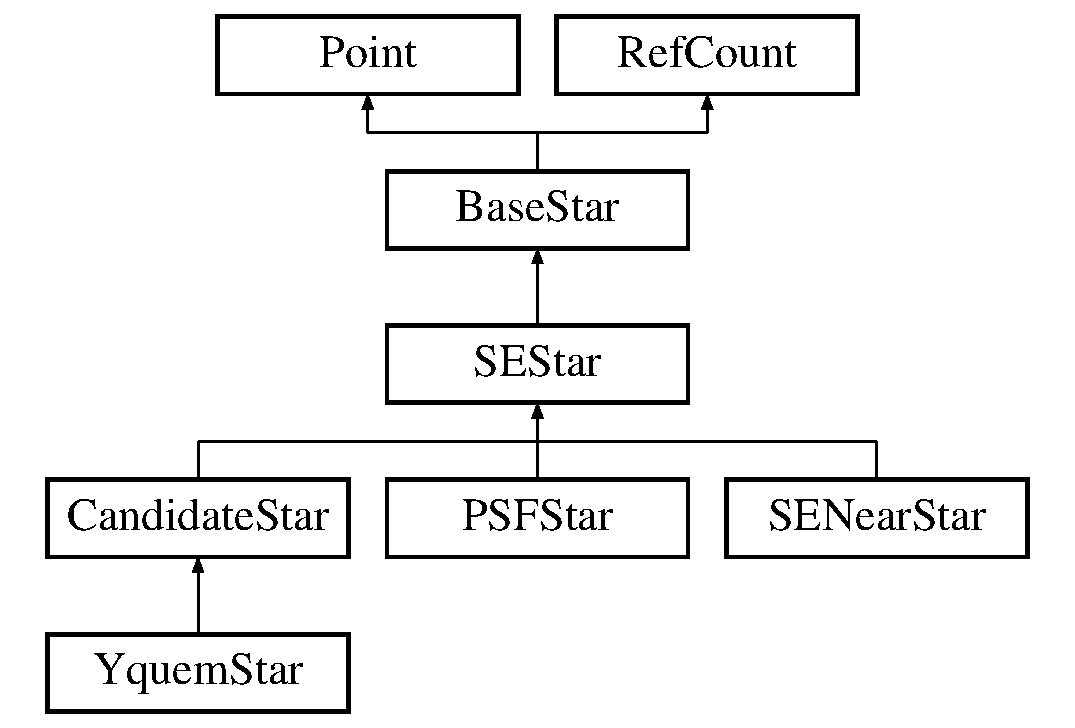
\includegraphics[height=5cm]{class_sestar}
\end{center}
\end{figure}
\subsubsection*{Public Methods}
\begin{CompactItemize}
\item 
\index{SEStar@{SEStar}!SEStar@{SEStar}}\index{SEStar@{SEStar}!SEStar@{SEStar}}
{\bf SEStar} ()\label{class_sestar_a0}

\item 
\index{SEStar@{SEStar}!SEStar@{SEStar}}\index{SEStar@{SEStar}!SEStar@{SEStar}}
{\bf SEStar} (double xx, double yy, double ff)\label{class_sestar_a1}

\item 
\index{HasNeighbours@{HasNeighbours}!SEStar@{SEStar}}\index{SEStar@{SEStar}!HasNeighbours@{Has\-Neighbours}}
bool {\bf Has\-Neighbours} () const\label{class_sestar_a2}

\begin{CompactList}\small\item\em The object has neighbours, bright and close enough to bias aperture photometry.\item\end{CompactList}\item 
\index{IsBlended@{IsBlended}!SEStar@{SEStar}}\index{SEStar@{SEStar}!IsBlended@{Is\-Blended}}
bool {\bf Is\-Blended} () const\label{class_sestar_a3}

\begin{CompactList}\small\item\em The object is blended with another one.\item\end{CompactList}\item 
\index{IsBad@{IsBad}!SEStar@{SEStar}}\index{SEStar@{SEStar}!IsBad@{Is\-Bad}}
bool {\bf Is\-Bad} () const\label{class_sestar_a4}

\item 
\index{IsCosmic@{IsCosmic}!SEStar@{SEStar}}\index{SEStar@{SEStar}!IsCosmic@{Is\-Cosmic}}
bool {\bf Is\-Cosmic} () const\label{class_sestar_a5}

\item 
\index{IsSaturated@{IsSaturated}!SEStar@{SEStar}}\index{SEStar@{SEStar}!IsSaturated@{Is\-Saturated}}
bool {\bf Is\-Saturated} (const double saturation) const\label{class_sestar_a6}

\begin{CompactList}\small\item\em at least one pixel is saturated.\item\end{CompactList}\item 
\index{IsSaturated@{IsSaturated}!SEStar@{SEStar}}\index{SEStar@{SEStar}!IsSaturated@{Is\-Saturated}}
bool {\bf Is\-Saturated} () const\label{class_sestar_a7}

\item 
\index{IsTruncated@{IsTruncated}!SEStar@{SEStar}}\index{SEStar@{SEStar}!IsTruncated@{Is\-Truncated}}
bool {\bf Is\-Truncated} () const\label{class_sestar_a8}

\begin{CompactList}\small\item\em the object is truncated.\item\end{CompactList}\item 
\index{FlagAsSaturated@{FlagAsSaturated}!SEStar@{SEStar}}\index{SEStar@{SEStar}!FlagAsSaturated@{Flag\-As\-Saturated}}
void {\bf Flag\-As\-Saturated} ()\label{class_sestar_a9}

\begin{CompactList}\small\item\em To flag a star as saturated.\item\end{CompactList}\item 
\index{FlagAsCosmic@{FlagAsCosmic}!SEStar@{SEStar}}\index{SEStar@{SEStar}!FlagAsCosmic@{Flag\-As\-Cosmic}}
void {\bf Flag\-As\-Cosmic} ()\label{class_sestar_a10}

\begin{CompactList}\small\item\em To flag a star as cosmic.\item\end{CompactList}\item 
\index{FlagAsNotSaturated@{FlagAsNotSaturated}!SEStar@{SEStar}}\index{SEStar@{SEStar}!FlagAsNotSaturated@{Flag\-As\-Not\-Saturated}}
void {\bf Flag\-As\-Not\-Saturated} ()\label{class_sestar_a11}

\begin{CompactList}\small\item\em To un-flag a star because it is not saturated.\item\end{CompactList}\item 
\index{X_Peak@{X\_\-Peak}!SEStar@{SEStar}}\index{SEStar@{SEStar}!X_Peak@{X\_\-Peak}}
double {\bf X\_\-Peak} () const\label{class_sestar_a12}

\begin{CompactList}\small\item\em x-coordinate of the brightest pixel.\item\end{CompactList}\item 
\index{Y_Peak@{Y\_\-Peak}!SEStar@{SEStar}}\index{SEStar@{SEStar}!Y_Peak@{Y\_\-Peak}}
double {\bf Y\_\-Peak} () const\label{class_sestar_a13}

\begin{CompactList}\small\item\em y-coordinate of the brightest pixel.\item\end{CompactList}\item 
\index{EFlux@{EFlux}!SEStar@{SEStar}}\index{SEStar@{SEStar}!EFlux@{EFlux}}
double {\bf EFlux} () const\label{class_sestar_a14}

\begin{CompactList}\small\item\em RMS error for BEST flux.\item\end{CompactList}\item 
\index{Fluxmax@{Fluxmax}!SEStar@{SEStar}}\index{SEStar@{SEStar}!Fluxmax@{Fluxmax}}
double {\bf Fluxmax} () const\label{class_sestar_a15}

\begin{CompactList}\small\item\em Peak flux $\ast$$\ast$above background$\ast$$\ast$.\item\end{CompactList}\item 
\index{Fond@{Fond}!SEStar@{SEStar}}\index{SEStar@{SEStar}!Fond@{Fond}}
double {\bf Fond} () const\label{class_sestar_a16}

\begin{CompactList}\small\item\em background.\item\end{CompactList}\item 
\index{Flux_aper@{Flux\_\-aper}!SEStar@{SEStar}}\index{SEStar@{SEStar}!Flux_aper@{Flux\_\-aper}}
double {\bf Flux\_\-aper} () const\label{class_sestar_a17}

\begin{CompactList}\small\item\em SExtractor FLUX\_\-AUTO: Flux within a Kron-like elliptical aperture.\item\end{CompactList}\item 
\index{Eflux_aper@{Eflux\_\-aper}!SEStar@{SEStar}}\index{SEStar@{SEStar}!Eflux_aper@{Eflux\_\-aper}}
double {\bf Eflux\_\-aper} () const\label{class_sestar_a18}

\begin{CompactList}\small\item\em SExtractor FLUXERR\_\-AUTO : RMS error for Flux\_\-aper.\item\end{CompactList}\item 
\index{Flux_fixaper@{Flux\_\-fixaper}!SEStar@{SEStar}}\index{SEStar@{SEStar}!Flux_fixaper@{Flux\_\-fixaper}}
double {\bf Flux\_\-fixaper} () const\label{class_sestar_a19}

\item 
\index{Eflux_fixaper@{Eflux\_\-fixaper}!SEStar@{SEStar}}\index{SEStar@{SEStar}!Eflux_fixaper@{Eflux\_\-fixaper}}
double {\bf Eflux\_\-fixaper} () const\label{class_sestar_a20}

\item 
\index{Flux_iso@{Flux\_\-iso}!SEStar@{SEStar}}\index{SEStar@{SEStar}!Flux_iso@{Flux\_\-iso}}
double {\bf Flux\_\-iso} () const\label{class_sestar_a21}

\begin{CompactList}\small\item\em SExtractor FLUX\_\-ISO: isophotal flux.\item\end{CompactList}\item 
\index{Eflux_iso@{Eflux\_\-iso}!SEStar@{SEStar}}\index{SEStar@{SEStar}!Eflux_iso@{Eflux\_\-iso}}
double {\bf Eflux\_\-iso} () const\label{class_sestar_a22}

\begin{CompactList}\small\item\em SExtractor FLUXERR\_\-ISO: error on isophotal flux.\item\end{CompactList}\item 
\index{Flux_isocor@{Flux\_\-isocor}!SEStar@{SEStar}}\index{SEStar@{SEStar}!Flux_isocor@{Flux\_\-isocor}}
double {\bf Flux\_\-isocor} () const\label{class_sestar_a23}

\begin{CompactList}\small\item\em SExtractor FLUX\_\-ISOCOR: isophotal corrected flux.\item\end{CompactList}\item 
\index{Eflux_isocor@{Eflux\_\-isocor}!SEStar@{SEStar}}\index{SEStar@{SEStar}!Eflux_isocor@{Eflux\_\-isocor}}
double {\bf Eflux\_\-isocor} () const\label{class_sestar_a24}

\begin{CompactList}\small\item\em SExtractor FLUXERR\_\-ISOCOR error on isophotal corrected flux.\item\end{CompactList}\item 
\index{Fwhm@{Fwhm}!SEStar@{SEStar}}\index{SEStar@{SEStar}!Fwhm@{Fwhm}}
double {\bf Fwhm} () const\label{class_sestar_a25}

\begin{CompactList}\small\item\em fwhm in pixels.\item\end{CompactList}\item 
\index{Kronradius@{Kronradius}!SEStar@{SEStar}}\index{SEStar@{SEStar}!Kronradius@{Kronradius}}
double {\bf Kronradius} () const\label{class_sestar_a26}

\begin{CompactList}\small\item\em extension of the aperture , in units of A or B.\item\end{CompactList}\item 
\index{Isoarea@{Isoarea}!SEStar@{SEStar}}\index{SEStar@{SEStar}!Isoarea@{Isoarea}}
double {\bf Isoarea} () const\label{class_sestar_a27}

\begin{CompactList}\small\item\em area of lowest isophote en pixels.\item\end{CompactList}\item 
\index{Mxx@{Mxx}!SEStar@{SEStar}}\index{SEStar@{SEStar}!Mxx@{Mxx}}
double {\bf Mxx} () const\label{class_sestar_a28}

\begin{CompactList}\small\item\em $<$\$x$^\wedge$2\$ - $<$x$>$\$\{\}$^\wedge$2\$$>$.\item\end{CompactList}\item 
\index{Myy@{Myy}!SEStar@{SEStar}}\index{SEStar@{SEStar}!Myy@{Myy}}
double {\bf Myy} () const\label{class_sestar_a29}

\begin{CompactList}\small\item\em $<$\$y$^\wedge$2\$ - $<$y$>$\$\{\}$^\wedge$2\$$>$.\item\end{CompactList}\item 
\index{Mxy@{Mxy}!SEStar@{SEStar}}\index{SEStar@{SEStar}!Mxy@{Mxy}}
double {\bf Mxy} () const\label{class_sestar_a30}

\begin{CompactList}\small\item\em $<$xy - $<$x$>$$<$y$>$$>$.\item\end{CompactList}\item 
\index{A@{A}!SEStar@{SEStar}}\index{SEStar@{SEStar}!A@{A}}
double {\bf A} () const\label{class_sestar_a31}

\begin{CompactList}\small\item\em Profile RMS along major axis.\item\end{CompactList}\item 
\index{B@{B}!SEStar@{SEStar}}\index{SEStar@{SEStar}!B@{B}}
double {\bf B} () const\label{class_sestar_a32}

\begin{CompactList}\small\item\em Profile RMS along minor axis.\item\end{CompactList}\item 
\index{Gyr_Angle@{Gyr\_\-Angle}!SEStar@{SEStar}}\index{SEStar@{SEStar}!Gyr_Angle@{Gyr\_\-Angle}}
double {\bf Gyr\_\-Angle} () const\label{class_sestar_a33}

\begin{CompactList}\small\item\em gyration angle of the major axis 0.0 = axis en degres Position angle.\item\end{CompactList}\item 
\index{Flag@{Flag}!SEStar@{SEStar}}\index{SEStar@{SEStar}!Flag@{Flag}}
int {\bf Flag} () const\label{class_sestar_a34}

\begin{CompactList}\small\item\em Extraction flags.\item\end{CompactList}\item 
\index{FlagBad@{FlagBad}!SEStar@{SEStar}}\index{SEStar@{SEStar}!FlagBad@{Flag\-Bad}}
int {\bf Flag\-Bad} () const\label{class_sestar_a35}

\begin{CompactList}\small\item\em number of bad pixels in iso area.\item\end{CompactList}\item 
\index{Cstar@{Cstar}!SEStar@{SEStar}}\index{SEStar@{SEStar}!Cstar@{Cstar}}
double {\bf Cstar} () const\label{class_sestar_a36}

\begin{CompactList}\small\item\em star/galaxy classification: [0=gal ... 1=star].\item\end{CompactList}\item 
\index{Xtrunc@{Xtrunc}!SEStar@{SEStar}}\index{SEStar@{SEStar}!Xtrunc@{Xtrunc}}
double {\bf Xtrunc} () const\label{class_sestar_a37}

\begin{CompactList}\small\item\em local barycenter (see Pierre).\item\end{CompactList}\item 
\index{Ytrunc@{Ytrunc}!SEStar@{SEStar}}\index{SEStar@{SEStar}!Ytrunc@{Ytrunc}}
double {\bf Ytrunc} () const\label{class_sestar_a38}

\begin{CompactList}\small\item\em local barycenter.\item\end{CompactList}\item 
\index{N@{N}!SEStar@{SEStar}}\index{SEStar@{SEStar}!N@{N}}
int {\bf N} () const\label{class_sestar_a39}

\item 
\index{Iter@{Iter}!SEStar@{SEStar}}\index{SEStar@{SEStar}!Iter@{Iter}}
int {\bf Iter} () const\label{class_sestar_a40}

\begin{CompactList}\small\item\em Number of iteration in the PSF fitting (ALLSTAR) procedure.\item\end{CompactList}\item 
\index{Chi@{Chi}!SEStar@{SEStar}}\index{SEStar@{SEStar}!Chi@{Chi}}
double {\bf Chi} () const\label{class_sestar_a41}

\begin{CompactList}\small\item\em chi from fit (to be plot vs. magnitude).\item\end{CompactList}\item 
\index{Sharp@{Sharp}!SEStar@{SEStar}}\index{SEStar@{SEStar}!Sharp@{Sharp}}
double {\bf Sharp} () const\label{class_sestar_a42}

\begin{CompactList}\small\item\em sharp diagnostic (to be plot vs. magnitude).\item\end{CompactList}\item 
\index{X_Peak@{X\_\-Peak}!SEStar@{SEStar}}\index{SEStar@{SEStar}!X_Peak@{X\_\-Peak}}
double\& {\bf X\_\-Peak} ()\label{class_sestar_a43}

\item 
\index{Y_Peak@{Y\_\-Peak}!SEStar@{SEStar}}\index{SEStar@{SEStar}!Y_Peak@{Y\_\-Peak}}
double\& {\bf Y\_\-Peak} ()\label{class_sestar_a44}

\item 
\index{EFlux@{EFlux}!SEStar@{SEStar}}\index{SEStar@{SEStar}!EFlux@{EFlux}}
double\& {\bf EFlux} ()\label{class_sestar_a45}

\item 
\index{Fluxmax@{Fluxmax}!SEStar@{SEStar}}\index{SEStar@{SEStar}!Fluxmax@{Fluxmax}}
double\& {\bf Fluxmax} ()\label{class_sestar_a46}

\item 
\index{Fond@{Fond}!SEStar@{SEStar}}\index{SEStar@{SEStar}!Fond@{Fond}}
double\& {\bf Fond} ()\label{class_sestar_a47}

\item 
\index{Flux_aper@{Flux\_\-aper}!SEStar@{SEStar}}\index{SEStar@{SEStar}!Flux_aper@{Flux\_\-aper}}
double\& {\bf Flux\_\-aper} ()\label{class_sestar_a48}

\item 
\index{Eflux_aper@{Eflux\_\-aper}!SEStar@{SEStar}}\index{SEStar@{SEStar}!Eflux_aper@{Eflux\_\-aper}}
double\& {\bf Eflux\_\-aper} ()\label{class_sestar_a49}

\item 
\index{Flux_fixaper@{Flux\_\-fixaper}!SEStar@{SEStar}}\index{SEStar@{SEStar}!Flux_fixaper@{Flux\_\-fixaper}}
double\& {\bf Flux\_\-fixaper} ()\label{class_sestar_a50}

\item 
\index{Eflux_fixaper@{Eflux\_\-fixaper}!SEStar@{SEStar}}\index{SEStar@{SEStar}!Eflux_fixaper@{Eflux\_\-fixaper}}
double\& {\bf Eflux\_\-fixaper} ()\label{class_sestar_a51}

\item 
\index{Flux_iso@{Flux\_\-iso}!SEStar@{SEStar}}\index{SEStar@{SEStar}!Flux_iso@{Flux\_\-iso}}
double\& {\bf Flux\_\-iso} ()\label{class_sestar_a52}

\item 
\index{Eflux_iso@{Eflux\_\-iso}!SEStar@{SEStar}}\index{SEStar@{SEStar}!Eflux_iso@{Eflux\_\-iso}}
double\& {\bf Eflux\_\-iso} ()\label{class_sestar_a53}

\item 
\index{Flux_isocor@{Flux\_\-isocor}!SEStar@{SEStar}}\index{SEStar@{SEStar}!Flux_isocor@{Flux\_\-isocor}}
double\& {\bf Flux\_\-isocor} ()\label{class_sestar_a54}

\item 
\index{Eflux_isocor@{Eflux\_\-isocor}!SEStar@{SEStar}}\index{SEStar@{SEStar}!Eflux_isocor@{Eflux\_\-isocor}}
double\& {\bf Eflux\_\-isocor} ()\label{class_sestar_a55}

\item 
\index{Fwhm@{Fwhm}!SEStar@{SEStar}}\index{SEStar@{SEStar}!Fwhm@{Fwhm}}
double\& {\bf Fwhm} ()\label{class_sestar_a56}

\item 
\index{Kronradius@{Kronradius}!SEStar@{SEStar}}\index{SEStar@{SEStar}!Kronradius@{Kronradius}}
double\& {\bf Kronradius} ()\label{class_sestar_a57}

\item 
\index{Isoarea@{Isoarea}!SEStar@{SEStar}}\index{SEStar@{SEStar}!Isoarea@{Isoarea}}
double\& {\bf Isoarea} ()\label{class_sestar_a58}

\item 
\index{Mxx@{Mxx}!SEStar@{SEStar}}\index{SEStar@{SEStar}!Mxx@{Mxx}}
double\& {\bf Mxx} ()\label{class_sestar_a59}

\item 
\index{Myy@{Myy}!SEStar@{SEStar}}\index{SEStar@{SEStar}!Myy@{Myy}}
double\& {\bf Myy} ()\label{class_sestar_a60}

\item 
\index{Mxy@{Mxy}!SEStar@{SEStar}}\index{SEStar@{SEStar}!Mxy@{Mxy}}
double\& {\bf Mxy} ()\label{class_sestar_a61}

\item 
\index{A@{A}!SEStar@{SEStar}}\index{SEStar@{SEStar}!A@{A}}
double\& {\bf A} ()\label{class_sestar_a62}

\item 
\index{B@{B}!SEStar@{SEStar}}\index{SEStar@{SEStar}!B@{B}}
double\& {\bf B} ()\label{class_sestar_a63}

\item 
\index{Gyr_Angle@{Gyr\_\-Angle}!SEStar@{SEStar}}\index{SEStar@{SEStar}!Gyr_Angle@{Gyr\_\-Angle}}
double\& {\bf Gyr\_\-Angle} ()\label{class_sestar_a64}

\item 
\index{Flag@{Flag}!SEStar@{SEStar}}\index{SEStar@{SEStar}!Flag@{Flag}}
int\& {\bf Flag} ()\label{class_sestar_a65}

\item 
\index{FlagBad@{FlagBad}!SEStar@{SEStar}}\index{SEStar@{SEStar}!FlagBad@{Flag\-Bad}}
int\& {\bf Flag\-Bad} ()\label{class_sestar_a66}

\item 
\index{Cstar@{Cstar}!SEStar@{SEStar}}\index{SEStar@{SEStar}!Cstar@{Cstar}}
double\& {\bf Cstar} ()\label{class_sestar_a67}

\item 
\index{Xtrunc@{Xtrunc}!SEStar@{SEStar}}\index{SEStar@{SEStar}!Xtrunc@{Xtrunc}}
double\& {\bf Xtrunc} ()\label{class_sestar_a68}

\item 
\index{Ytrunc@{Ytrunc}!SEStar@{SEStar}}\index{SEStar@{SEStar}!Ytrunc@{Ytrunc}}
double\& {\bf Ytrunc} ()\label{class_sestar_a69}

\item 
\index{N@{N}!SEStar@{SEStar}}\index{SEStar@{SEStar}!N@{N}}
int\& {\bf N} ()\label{class_sestar_a70}

\item 
\index{Iter@{Iter}!SEStar@{SEStar}}\index{SEStar@{SEStar}!Iter@{Iter}}
int\& {\bf Iter} ()\label{class_sestar_a71}

\item 
\index{Chi@{Chi}!SEStar@{SEStar}}\index{SEStar@{SEStar}!Chi@{Chi}}
double\& {\bf Chi} ()\label{class_sestar_a72}

\item 
\index{Sharp@{Sharp}!SEStar@{SEStar}}\index{SEStar@{SEStar}!Sharp@{Sharp}}
double\& {\bf Sharp} ()\label{class_sestar_a73}

\item 
\index{dumpn@{dumpn}!SEStar@{SEStar}}\index{SEStar@{SEStar}!dumpn@{dumpn}}
virtual void {\bf dumpn} (ostream \&s=cout) const\label{class_sestar_a74}

\begin{CompactList}\small\item\em for dump with NO end-of-line.\item\end{CompactList}\item 
\index{dump@{dump}!SEStar@{SEStar}}\index{SEStar@{SEStar}!dump@{dump}}
virtual void {\bf dump} (ostream \&s=cout) const\label{class_sestar_a75}

\begin{CompactList}\small\item\em for dump.\item\end{CompactList}\item 
\index{writen@{writen}!SEStar@{SEStar}}\index{SEStar@{SEStar}!writen@{writen}}
virtual void {\bf writen} (ostream \&s=cout) const\label{class_sestar_a76}

\begin{CompactList}\small\item\em for write with NO end-of-line.\item\end{CompactList}\item 
\index{read_it@{read\_\-it}!SEStar@{SEStar}}\index{SEStar@{SEStar}!read_it@{read\_\-it}}
virtual void {\bf read\_\-it} (istream \&r, const char $\ast$Format)\label{class_sestar_a77}

\begin{CompactList}\small\item\em to read once the object is created.\item\end{CompactList}\item 
\index{WriteHeader_@{WriteHeader\_\-}!SEStar@{SEStar}}\index{SEStar@{SEStar}!WriteHeader_@{Write\-Header\_\-}}
std::string {\bf Write\-Header\_\-} (ostream \&pr=cout, const char $\ast$i=NULL) const\label{class_sestar_a78}

\item 
\index{IsOK@{IsOK}!SEStar@{SEStar}}\index{SEStar@{SEStar}!IsOK@{Is\-OK}}
bool {\bf Is\-OK} (const double \&saturation) const\label{class_sestar_a79}

\end{CompactItemize}
\subsubsection*{Static Public Methods}
\begin{CompactItemize}
\item 
\index{read@{read}!SEStar@{SEStar}}\index{SEStar@{SEStar}!read@{read}}
SEStar$\ast$ {\bf read} (istream \&r, const char $\ast$Format)\label{class_sestar_d0}

\begin{CompactList}\small\item\em to read and create the object.\item\end{CompactList}\item 
\index{TypeName@{TypeName}!SEStar@{SEStar}}\index{SEStar@{SEStar}!TypeName@{Type\-Name}}
const char$\ast$ {\bf Type\-Name} ()\label{class_sestar_d1}

\end{CompactItemize}
\subsubsection*{Protected Attributes}
\begin{CompactItemize}
\item 
\index{num@{num}!SEStar@{SEStar}}\index{SEStar@{SEStar}!num@{num}}
int {\bf num}\label{class_sestar_n0}

\item 
\index{xpeak@{xpeak}!SEStar@{SEStar}}\index{SEStar@{SEStar}!xpeak@{xpeak}}
double {\bf xpeak}\label{class_sestar_n1}

\item 
\index{ypeak@{ypeak}!SEStar@{SEStar}}\index{SEStar@{SEStar}!ypeak@{ypeak}}
double {\bf ypeak}\label{class_sestar_n2}

\item 
\index{fluxmax@{fluxmax}!SEStar@{SEStar}}\index{SEStar@{SEStar}!fluxmax@{fluxmax}}
double {\bf fluxmax}\label{class_sestar_n3}

\item 
\index{e_flux@{e\_\-flux}!SEStar@{SEStar}}\index{SEStar@{SEStar}!e_flux@{e\_\-flux}}
double {\bf e\_\-flux}\label{class_sestar_n4}

\item 
\index{fond@{fond}!SEStar@{SEStar}}\index{SEStar@{SEStar}!fond@{fond}}
double {\bf fond}\label{class_sestar_n5}

\item 
\index{flux_aper@{flux\_\-aper}!SEStar@{SEStar}}\index{SEStar@{SEStar}!flux_aper@{flux\_\-aper}}
double {\bf flux\_\-aper}\label{class_sestar_n6}

\item 
\index{e_flux_aper@{e\_\-flux\_\-aper}!SEStar@{SEStar}}\index{SEStar@{SEStar}!e_flux_aper@{e\_\-flux\_\-aper}}
double {\bf e\_\-flux\_\-aper}\label{class_sestar_n7}

\item 
\index{flux_fixaper@{flux\_\-fixaper}!SEStar@{SEStar}}\index{SEStar@{SEStar}!flux_fixaper@{flux\_\-fixaper}}
double {\bf flux\_\-fixaper}\label{class_sestar_n8}

\item 
\index{e_flux_fixaper@{e\_\-flux\_\-fixaper}!SEStar@{SEStar}}\index{SEStar@{SEStar}!e_flux_fixaper@{e\_\-flux\_\-fixaper}}
double {\bf e\_\-flux\_\-fixaper}\label{class_sestar_n9}

\item 
\index{flux_iso@{flux\_\-iso}!SEStar@{SEStar}}\index{SEStar@{SEStar}!flux_iso@{flux\_\-iso}}
double {\bf flux\_\-iso}\label{class_sestar_n10}

\item 
\index{e_flux_iso@{e\_\-flux\_\-iso}!SEStar@{SEStar}}\index{SEStar@{SEStar}!e_flux_iso@{e\_\-flux\_\-iso}}
double {\bf e\_\-flux\_\-iso}\label{class_sestar_n11}

\item 
\index{flux_isocor@{flux\_\-isocor}!SEStar@{SEStar}}\index{SEStar@{SEStar}!flux_isocor@{flux\_\-isocor}}
double {\bf flux\_\-isocor}\label{class_sestar_n12}

\item 
\index{e_flux_isocor@{e\_\-flux\_\-isocor}!SEStar@{SEStar}}\index{SEStar@{SEStar}!e_flux_isocor@{e\_\-flux\_\-isocor}}
double {\bf e\_\-flux\_\-isocor}\label{class_sestar_n13}

\item 
\index{kronradius@{kronradius}!SEStar@{SEStar}}\index{SEStar@{SEStar}!kronradius@{kronradius}}
double {\bf kronradius}\label{class_sestar_n14}

\item 
\index{isoarea@{isoarea}!SEStar@{SEStar}}\index{SEStar@{SEStar}!isoarea@{isoarea}}
double {\bf isoarea}\label{class_sestar_n15}

\item 
\index{fwhm@{fwhm}!SEStar@{SEStar}}\index{SEStar@{SEStar}!fwhm@{fwhm}}
double {\bf fwhm}\label{class_sestar_n16}

\item 
\index{mxx@{mxx}!SEStar@{SEStar}}\index{SEStar@{SEStar}!mxx@{mxx}}
double {\bf mxx}\label{class_sestar_n17}

\item 
\index{myy@{myy}!SEStar@{SEStar}}\index{SEStar@{SEStar}!myy@{myy}}
double {\bf myy}\label{class_sestar_n18}

\item 
\index{mxy@{mxy}!SEStar@{SEStar}}\index{SEStar@{SEStar}!mxy@{mxy}}
double {\bf mxy}\label{class_sestar_n19}

\item 
\index{a@{a}!SEStar@{SEStar}}\index{SEStar@{SEStar}!a@{a}}
double {\bf a}\label{class_sestar_n20}

\item 
\index{b@{b}!SEStar@{SEStar}}\index{SEStar@{SEStar}!b@{b}}
double {\bf b}\label{class_sestar_n21}

\item 
\index{gyr_angle@{gyr\_\-angle}!SEStar@{SEStar}}\index{SEStar@{SEStar}!gyr_angle@{gyr\_\-angle}}
double {\bf gyr\_\-angle}\label{class_sestar_n22}

\item 
\index{flag@{flag}!SEStar@{SEStar}}\index{SEStar@{SEStar}!flag@{flag}}
int {\bf flag}\label{class_sestar_n23}

\item 
\index{flagbad@{flagbad}!SEStar@{SEStar}}\index{SEStar@{SEStar}!flagbad@{flagbad}}
int {\bf flagbad}\label{class_sestar_n24}

\item 
\index{cstar@{cstar}!SEStar@{SEStar}}\index{SEStar@{SEStar}!cstar@{cstar}}
double {\bf cstar}\label{class_sestar_n25}

\item 
\index{xtrunc@{xtrunc}!SEStar@{SEStar}}\index{SEStar@{SEStar}!xtrunc@{xtrunc}}
double {\bf xtrunc}\label{class_sestar_n26}

\item 
\index{ytrunc@{ytrunc}!SEStar@{SEStar}}\index{SEStar@{SEStar}!ytrunc@{ytrunc}}
double {\bf ytrunc}\label{class_sestar_n27}

\item 
\index{iter@{iter}!SEStar@{SEStar}}\index{SEStar@{SEStar}!iter@{iter}}
int {\bf iter}\label{class_sestar_n28}

\item 
\index{chi@{chi}!SEStar@{SEStar}}\index{SEStar@{SEStar}!chi@{chi}}
double {\bf chi}\label{class_sestar_n29}

\item 
\index{sharp@{sharp}!SEStar@{SEStar}}\index{SEStar@{SEStar}!sharp@{sharp}}
double {\bf sharp}\label{class_sestar_n30}

\end{CompactItemize}


\subsubsection{Detailed Description}
SExtractor star.

The flux of {\bf Base\-Star} {\rm (p.\,\pageref{class_basestar})} is FLUX\_\-BEST from SExtractor, i.e. FLUX\_\-ISOCOR if not crowded, FLUX\_\-AUTO otherwise. 



The documentation for this class was generated from the following files:\begin{CompactItemize}
\item 
{\bf sestar.h}\item 
sestar.cc\end{CompactItemize}
